\documentclass[a4paper,12pt]{article}
\usepackage[utf8]{inputenc}
\usepackage[francais]{babel} 
\usepackage{listings}
\usepackage{textcomp}
\usepackage{color}
\usepackage{graphicx}
\usepackage{pdflscape}
\usepackage[colorlinks=false, urlcolor=black, breaklinks, pagebackref, citebordercolor={0 0 0}, filebordercolor={0 0 0}, linkbordercolor={0 0 0}, pagebordercolor={0 0 0}, runbordercolor={0 0 0}, urlbordercolor={0 0 0}, pdfborder={0 0 0}]{hyperref}

\lstset {
language=php,
upquote=true,
columns=flexible,
stringstyle=\ttfamily,
aboveskip=\topsep,
belowskip=\topsep,
breaklines,
breakindent=1.2em,
showstringspaces=false,
numbers=none,
frameshape={RYRYNYYYY}{yny}{yny}{RYRYNYYYY}
%frame=shadowbox,
%rulesepcolor=\color{black}
}

\setlength{\parskip}{10pt}

\title{\textbf{UMDN3E - Java - Paddle Game}}
\author{\textsc{Macky Dieng \& Baptiste Vannesson}}
\date{\textit{\today}}

\begin{document}

\begin{figure}
 \begin{center}
  
\includegraphics[scale=.3]{unicaen.png}
 \end{center}
\end{figure}

\maketitle

\begin{figure}[!h]
 \begin{center}
  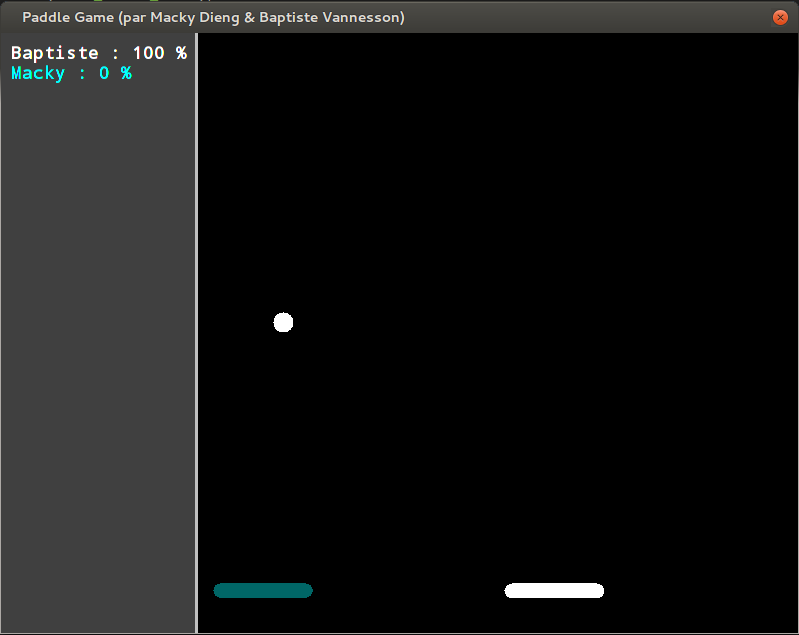
\includegraphics[scale=.3]{paddle-game.png}
 \end{center}
\end{figure}

\tableofcontents
\newpage

\section{Quelques précisions}

Ce projet a été développé sous Eclipse avec une architecture «~maison~». Les tâches de compilation, de distribution et de génération de la Javadoc ont été réalisées avec Ant par le biais d'un build.xml. Ce projet contient en réalité deux sous-projets (le client et le serveur) avec la structure suivante :

\begin{figure}[h]
 \begin{center}
  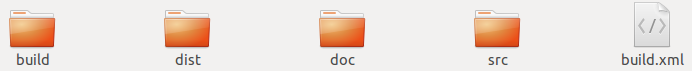
\includegraphics[scale=.5]{dossiers.png}
 \end{center}
 \caption{Structure d'un sous-projet}
\end{figure}

\vspace{7pt}

\begin{itemize}
 \item{« build » : contient les fichiers compilés (*.class).}
 \item{« dist » : contient le jar exécutable (cf. « java -jar *.jar »).}
 \item{« doc » : contient la Javadoc pour l'ensemble du code (cf. index.html).}
 \item{« src » : contient les sources d'un sous-projet, organisées en 3 packages.}
\end{itemize}

\vspace{7pt}

\textbf{
  À noter qu'il s'agit ici d'un projet réalisé en binôme. Pour ce devoir, la répartition était assez naturelle :
  \vspace{7pt}
  \begin{itemize}
    \item{Client : Baptiste}
    \item{Serveur : Macky}
  \end{itemize}
\end{textbf}
}

\vspace{10pt}

Bien évidemment, les phases de compréhension et de conception ont été menées à deux pour que chacun ait une vision globale du sujet et du fonctionnement de l'application. L'analyse du problème, de même que les diagrammes, de classes et de séquence, résultent donc d'un travail collectif. Pour le reste, tout ce qui a trait explicitement au \textbf{client} est à attribuer à \textbf{Baptiste}, et tout ce qui a trait explicitement au \textbf{serveur} est à attribuer à \textbf{Macky}. Ceci est valable pour les sections de ce rapport, mais aussi dans le code. Chaque classe indique son auteur dans la Javadoc. Naturellement, le protocole est une partie commune car c'est ce qui fait le lien entre le client et le serveur.

\textit{Le code étant largement documenté, ce rapport se contentera d'apporter un éclairage sur les points importants de la conception et du développement.}

\newpage

\section{Analyse du problème}

\subsection{Physique de la balle}

Pour gérer le déplacement d'une balle dans un plan, il y a plusieurs possibilités. Une première méthode consisterait à utiliser la trigonométrie pour déterminer les angles régissant la direction de la balle. Une deuxième méthode, plus simple, consiste en l'inversion d'un vecteur constant (norme fixe) de déplacement sous certaines conditions ; en l'occurrence lors d'une collision avec un mur ou une raquette.

\begin{figure}[h]
 \begin{center}
  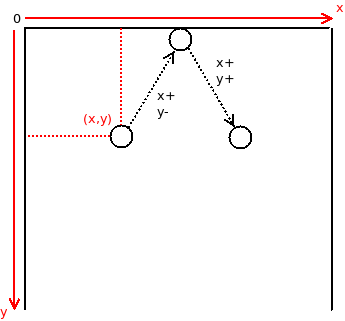
\includegraphics[scale=.5]{balle.png}
 \end{center}
 \caption{Rebond d'une balle dans un plan}
\end{figure}

Nous pourrions partir du principe qu'une balle peut naïvement sortir de l'espace de jeu, auquel cas il faudrait répercuter la distance en dehors du jeu à l'intérieur de celui-ci pour avoir un rebond correct. Mais nous pouvons aussi considérer qu'une balle ne doit jamais sortir de l'espace de jeu, et que par conséquent, il faut inverser le sens de déplacement de la balle, dès lors qu'elle s'apprête à toucher un mur. Pour cela on peut très bien utiliser deux booléens (un pour x, un pour y), qui vont permettre de savoir quand incrémenter, quand décrémenter, et sur quel axe.

En effet, une balle ne peut se déplacer que vers la gauche (-) ou vers la droite (+) sur l'axe des x, et vers le haut (-) ou vers le bas (+) sur l'axe des y. Les différentes combinaisons permises par ces deux booléens rendent possible un déplacement de la balle dans toutes les directions. Et dès que la balle se rapproche asymptotiquement d'un mur (\textless{} 1 px), on met à jour le booléen correspondant pour qu'elle reparte dans l'autre sens.

Le mur du bas étant absent, la balle sera perdue si son y devient supérieur au y des raquettes ; raquettes qui peuvent elles-mêmes être considérées comme des mini-murs. Le booléen propre à y est alors mis à jour si la balle touche une raquette, afin qu'elle rebondisse.

\subsection{Calcul des scores}

Calculer un score en temps réel dans le cadre d'un jeu multijoueur en réseau est probablement plus complexe qu'il n'y paraît de prime abord. Le calcul mathématique est relativement simple, puisqu'il s'agit d'un banal pourcentage. Mais le calcul des scores sous-entend plusieurs difficultés. Tout d'abord, avant tout calcul, il faut déterminer qui a marqué le point...

Pour ce faire, lorsqu'une collision est détectée (c'est-à-dire lorsque le x et le y de la balle rencontrent un x et un y d'une raquette), on détermine l'écart minimum (en valeur absolue) entre le x de la balle et le centre de la raquette de chaque joueur. La valeur absolue est ici essentielle car la balle peut arriver par la gauche ou par la droite. Or si on fait la différence entre le x de la balle et le centre de la raquette, on aura une valeur négative dans le premier cas et une valeur positive dans l'autre, alors que les distances sont potentiellement identiques.

\begin{figure}[h]
 \begin{center}
  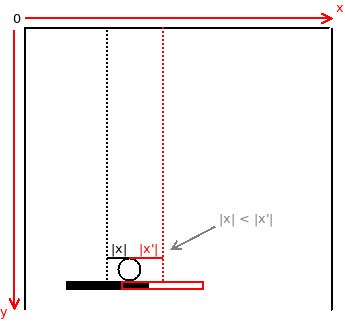
\includegraphics[scale=.5]{collision.png}
 \end{center}
 \caption{Détection de la collision la plus centrée}
\end{figure}

Une fois que la raquette la plus proche est déterminée, on part du principe que le joueur en question marque un nombre de points égal au nombre de joueurs en présence, y compris lui. Pour obtenir son score, il faut maintenant diviser le total des points qu'il a obtenus par le total des points idéal qu'il aurait pu avoir s'il avait tapé dans toutes les balles. On obtient ainsi un score entre 0 et 1. Par exemple, s'il y a deux joueurs et que le premier joueur a tapé dans toutes les balles, le premier joueur a un score de 1 et le deuxième de 0. L'affichage en pourcentage étant plus agréable, on peut ici multiplier par 100 et dire que le joueur 1 a un score de 100 \%, tandis que le joueur 2 a un score de 0 \%.

Cependant, un problème se pose... Imaginons qu'un joueur joue tout seul pendant une heure, avec 300 balles tapées. Lorsqu'un nouveau joueur se connecte, il ne faut pas que le nombre de points idéal soit déterminé à partir de celui du premier joueur. En effet, dans un tel cas de figure, si le nouveau joueur tape dans la balle, il n'aura pas un score de 100 \%, mais bien de (2 / 302) * 100, soit même pas 1 \%. 2 correspond ici au nombre de joueurs et 302 au nombre de points marqués depuis le début du jeu.

Pour avoir un calcul de score cohérent, il faut donc maintenir pour chaque joueur un compteur de points qu'il a marqués (correspondant au numérateur dans la division) et un compteur de points idéal depuis qu'il s'est connecté au jeu (correspondant au dénominateur dans la division). Ainsi le dénominateur connaît une progression à chaque collision, quel que soit le joueur, tandis que le numérateur peut rester figé si le joueur ne touche aucune balle. Évidemment, si personne ne touche la balle et que celle-ci tombe en dessous des raquettes, le dénominateur est tout de même incrémenté pour que chacun soit sanctionné (dans ce cas le numérateur ne change pas pour tous les joueurs).

Faisons une simulation simple par écrit, en prenant par exemple le scénario suivant :
\begin{enumerate}
  \item{Le joueur 1 se connecte et tape une première fois dans la balle.}
  \item{Le joueur 1 continue à jouer seul et rate le deuxième rebond.}
  \item{Le joueur 2 se connecte et remporte le premier point.}
  \item{Le joueur 3 se connecte et rate son premier point, remporté par le joueur 1.}
  \item{La balle tombe en dessous des raquettes}
\end{enumerate}

\newpage

\begin{tabular}{|c|c|c|c|}
    \hline
    Étape & Joueur 1 (score) & Joueur 2 (score) & Joueur 3 (score) \\
    \hline
    1 & (1/1) * 100 = 100 \% & - & - \\
    \hline
    2 & (1/2) * 100 = 50 \% & - & - \\
    \hline
    3 & (1/4) * 100 = 25 \% & (2/2) * 100 = 100 \% & - \\
    \hline
    4 & (4/7) * 100 = 57 \% & (2/5) * 100 = 40 \% & (0/3) * 100 = 0 \% \\
    \hline
    5 & (4/10) * 100 = 40 \% & (2/8) * 100 = 25 \% & (0/6) * 100 = 0 \% \\
    \hline
\end{tabular}

\section{Détails sur la conception}

\textbf{Attention} : les constructeurs, les accesseurs et les mutateurs n'apparaissent pas, volontairement, dans les diagrammes UML à des fins de simplification. Ils n'apporteraient pas grand-chose dans la représentation du problème et ne feraient qu'alourdir inutilement les diagrammes.

\subsection{Client}

Côté client, en dépit de l'aspect minimaliste du jeu, il y a un grand nombre de classes qui interviennent pour faire fonctionner l'application. Commençons d'abord par évoquer les éléments d'interface, c'est-à-dire la vue. Nous parlerons ensuite du projet sous un angle plus technique, en insistant notamment sur le multithreading.

L'affichage repose en premier lieu sur une JFrame qui nous sert ici de top-level container. Cette fenêtre est composée de deux panneaux, dont un JScrollPane (ScoresZone) qui contient une JList (ScoresList) pour l'affichage des scores, et un JPanel (GameZone) qui sert en quelque sorte d'ardoise pour dessiner les différents composants du jeu, en l'occurrence la balle et les raquettes (cf. paintComponent). Le principe ici est de faire un repaint() dès lors qu'une action se produit ; par exemple lorsque la balle bouge ou lorsque l'utilisateur déplace sa raquette. Dans le cas présent, d'après les principes du pattern \textbf{Observer}, c'est la zone de jeu (GameZone) qui s'écoute elle-même pour intercepter les événements propres au déplacement de la raquette, lancés par un MouseMotionListener.

On remarquera que les scores, et donc la JList (vue), s'appuient sur un modèle de liste ; en particulier un DefaultListModel. Il s'agit là d'une implémentation à échelle réduite du pattern \textbf{MVC} car, dans le cadre du jeu, nous pouvons facilement manipuler le modèle de liste (pour ajouter, modifier, supprimer des éléments) et en informer implicitement la vue ; toujours selon les principes du pattern \textbf{Observer}. En d'autres termes, à chaque fois que le modèle de liste est mis à jour, la JList se met à jour également et affiche l'état courant du modèle. D'un autre côté, notre JList étendue implémente indirectement l'interface ListCellRenderer, ceci afin de personnaliser l'affichage (ce qui s'avère notamment utile pour affecter une couleur spécifique à chaque label de la liste...).

On remarquera aussi l'utilisation du pattern \textbf{Singleton} pour s'assurer de ne manipuler qu'une seule instance de Ball. En effet, on part du principe que le jeu ne doit contenir qu'une seule balle. Il vaut donc mieux passer par une factory method statique (getBall) qui va s'assurer de l'inexistence de l'instance avant d'en créer une nouvelle, plutôt que par un constructeur public qui va recréer systématiquement une nouvelle instance. On sait d'ailleurs que les coordonnées de la balle sont fournies au client par le serveur, ce qui sous-entend des opérations fréquentes sur l'objet balle (dans des boucles infinies...). Le Singleton apporte ici une sécurité importante car un «~new~» dans une boucle infinie peut réellement avoir des effets inattendus !

Concernant maintenant le multithreading, on peut voir sur le diagramme UML du client qu'il y a 3 threads utilisés pour faire tourner l'application. Le premier thread est ClientGUI lui-même. Ce dernier se charge de récupérer les entrées/sorties pour interagir avec le serveur et de lancer deux threads qui vont s'occuper réellement de la communication. Le thread Input va gérer en continu tous les messages qui arrivent en entrée, c'est-à-dire tout ce qui vient du serveur, tandis que le thread Output va gérer en continu les messages à envoyer au serveur. En quelque sorte, ces deux derniers threads permettent une communication bidirectionnelle selon un protocole que nous verrons plus loin dans ce rapport.

On peut voir que les classes Input et Output héritent toutes les deux d'une classe abstraite IO. Cette classe abstraite est ici à des fins de factorisation, pour éviter la redondance de code. On sait en effet que les entrées/sorties dépendent directement de la zone de jeu. Par exemple, on met bien à jour la position de la balle dans la zone de jeu avec les données qui viennent du serveur (Input), et on envoie bien au serveur la nouvelle position de la raquette dans la zone de jeu (Ouput).

\begin{landscape}
  \begin{figure}
  \begin{center}
    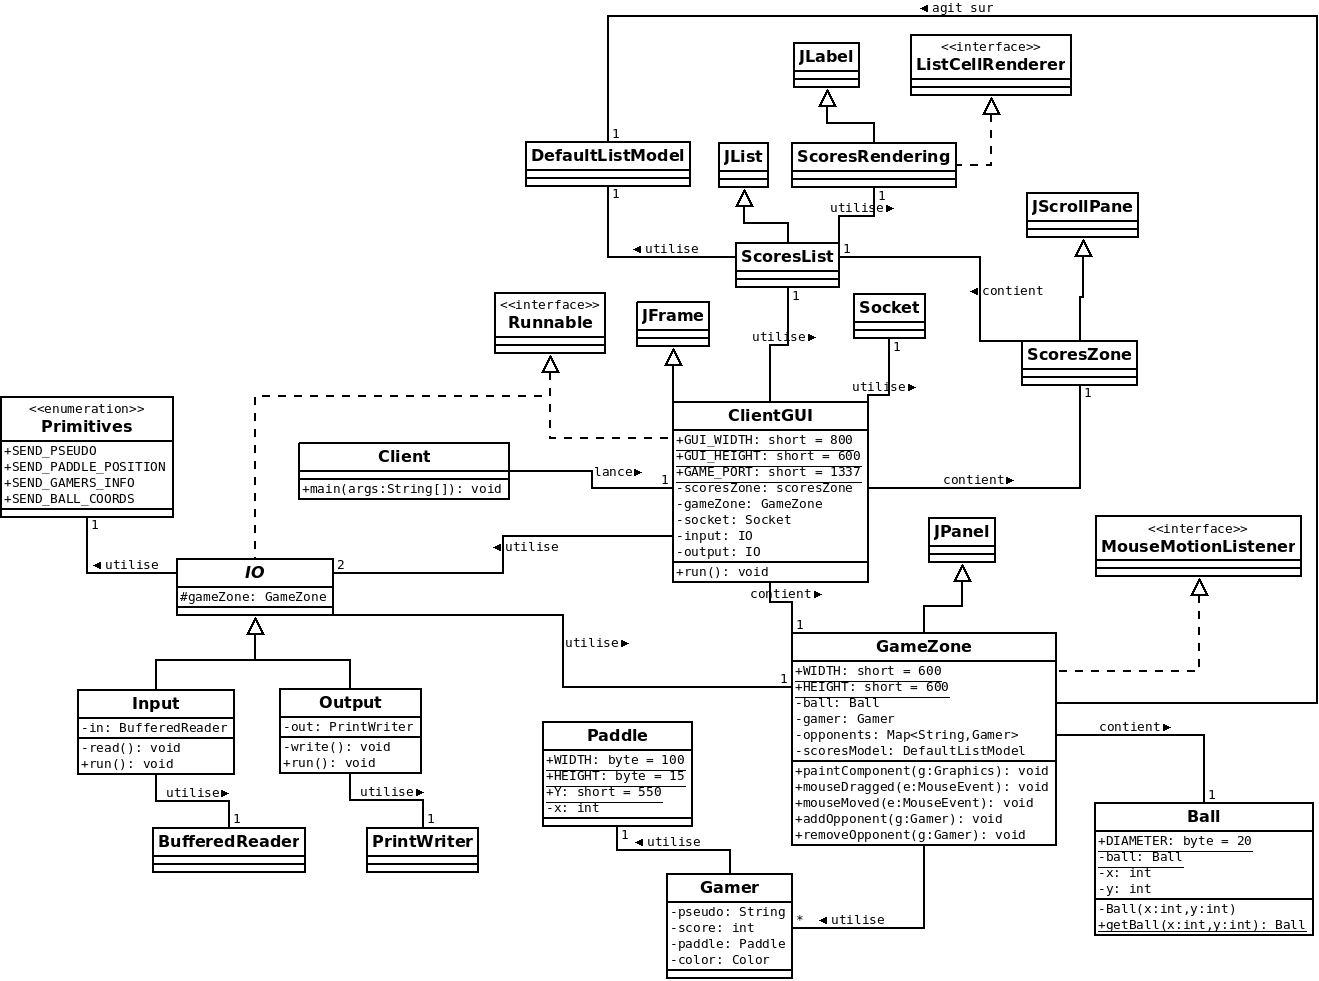
\includegraphics[scale=.4]{diagramme-client.png}
  \end{center}
  \caption{Diagramme de classes (UML) du client}
  \end{figure}
\end{landscape}

\subsection{Serveur}

Ce jeu s'appuie sur une architecture dite «~en étoile~». Le serveur est donc au centre, et tous les clients communiquent avec ce même serveur en même temps. De ce fait, le serveur a une très grande responsabilité quant à la reconnaissance des clients qui se connectent et à leur approvisionnement en informations.

Effectivement, il s'agit ici d'un jeu multijoueur en temps réel, c'est-à-dire que les joueurs se connectent, envoient leurs informations (pseudo, raquette, ...) ; et en retour le serveur leur renvoie (à tous) un certain nombre d'informations (position de la balle, position des raquettes de tous les joueurs, ainsi que les scores de tout le monde). Dans le cas présent, toute la partie métier est gérée par des threads. 

Pour développer l'application, il nous a fallu partir à la base d'une conception modulable. En regardant le diagramme de classe du serveur, on remarque la présence de la classe Server, qui est la classe principale du serveur, dont l'unique rôle est la réception des connexions clientes. Le serveur écoute en continu les connexions entrantes dans son thread principal, et une fois le client connecté, il délègue sa gestion à un thread (cf. GamerManagement). En restant sur le diagramme UML, on remarque que GamerManagement utilise un socket correspondant au socket du client qui vient de se connecter ; et donc à chaque client correspond un gestionnaire spécifique. On peut aussi voir que la classe Server possède une liste de références vers GamerManagement. Cette structure permet justement au serveur de retenir tout au long du jeu la liste des clients connectés, avec leurs informations respectives.

Le gestionnaire de clients (GamerManagement), qui est un thread, contient tout d'abord des références vers les entrées/sorties (in/out) du client qu'il gère via son socket. De plus, chaque GamerManagement utilise un objet Gamer représentant réellement l'entité client. Le but de cette association est de mémoriser toutes les informations du client (pseudo, position de la raquette, score et points) dans un objet réutilisable.

Enfin les threads Input et Output représentent respectivement les gestionnaires d'entrée et de sortie standard pour chaque client. Le thread Input va s'occuper de lire en continu les informations provenant de son client, tandis que le thread Output va s'occuper de l'envoi des données en continu à son client. C'est d'ailleurs ce thread (Output) qui est chargé du déplacement de la balle (celle-ci étant un \textbf{Singleton}) et du calcul des scores.

\begin{landscape}
  \begin{figure}
  \begin{center}
    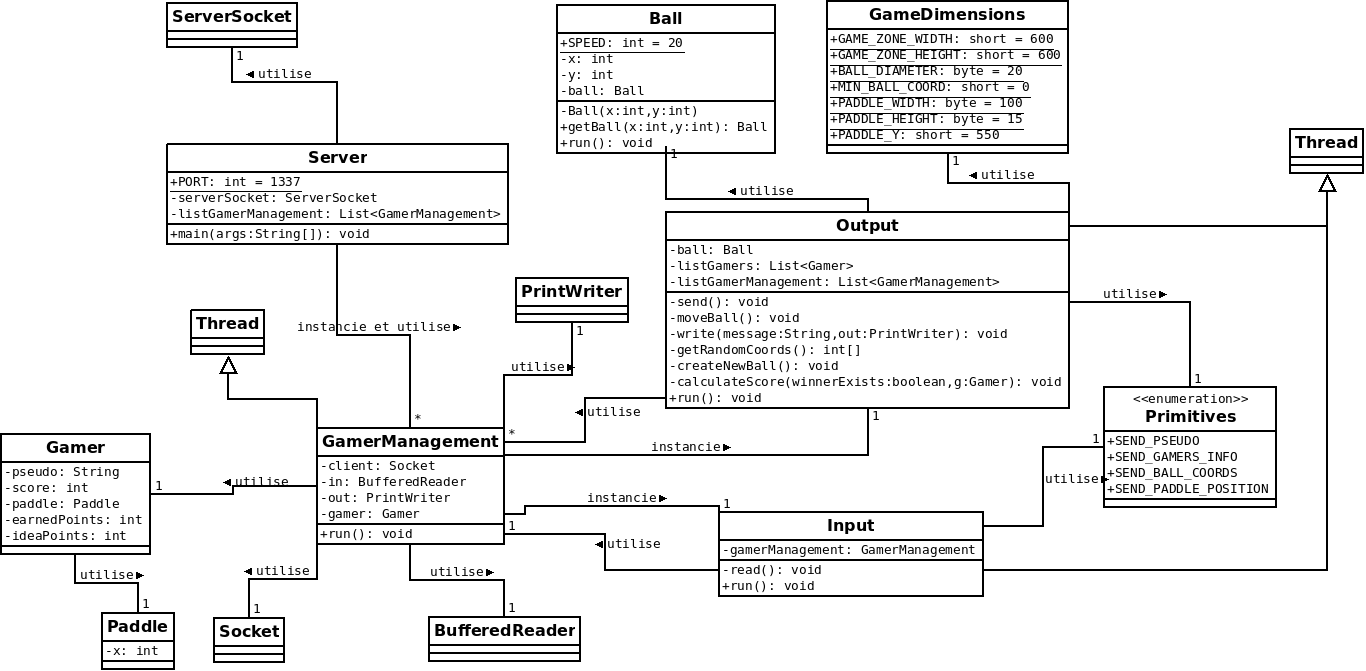
\includegraphics[scale=.4]{diagramme-serveur.png}
  \end{center}
  \caption{Diagramme de classes (UML) du serveur}
  \end{figure}
\end{landscape}

\subsection{Protocole}

Nous devions ici développer une application réseau de type client-serveur. Avant de commencer le développement, il était donc essentiel de concevoir le protocole, c'est-à-dire les règles de communication entre les deux acteurs de l'application.

\textbf{Le client doit envoyer au serveur :}
\begin{itemize}
 \item{Son pseudo}
 \item{La position de sa raquette}
\end{itemize}

\vspace{7pt}

\textbf{Le serveur doit envoyer au client :}
\begin{itemize}
 \item{Les informations sur tous les joueurs (pseudonymes, scores, positions des raquettes)}
 \item{La position de la balle}
\end{itemize}

\vspace{7pt}

En partant de ce constat, on peut ici définir quatre primitives pour régir la relation entre le client et le serveur :

\begin{itemize}
 \item{SEND\_PSEUDO}
 \item{SEND\_PADDLE\_POSITION}
 \item{SEND\_GAMERS\_INFO}
 \item{SEND\_BALL\_COORDS}
\end{itemize}

Ainsi, lorsque le client enverra la primitive SEND\_PSEUDO, le serveur comprendra que les données qui suivent contiennent le pseudo du joueur. De même, lorsque le serveur enverra la primitive SEND\_BALL\_COORDS, le client comprendra que le serveur lui envoie la nouvelle position de la balle. La communication entre le client et le serveur est désormais possible.

\begin{figure}[!h]
  \begin{center}
    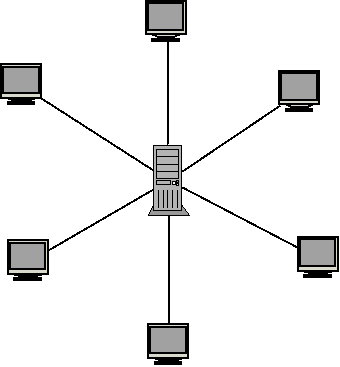
\includegraphics[scale=.3]{architecture.png}
  \end{center}
  \caption{Architecture en étoile}
\end{figure}

\newpage

\begin{figure}[!h]
  \begin{center}
    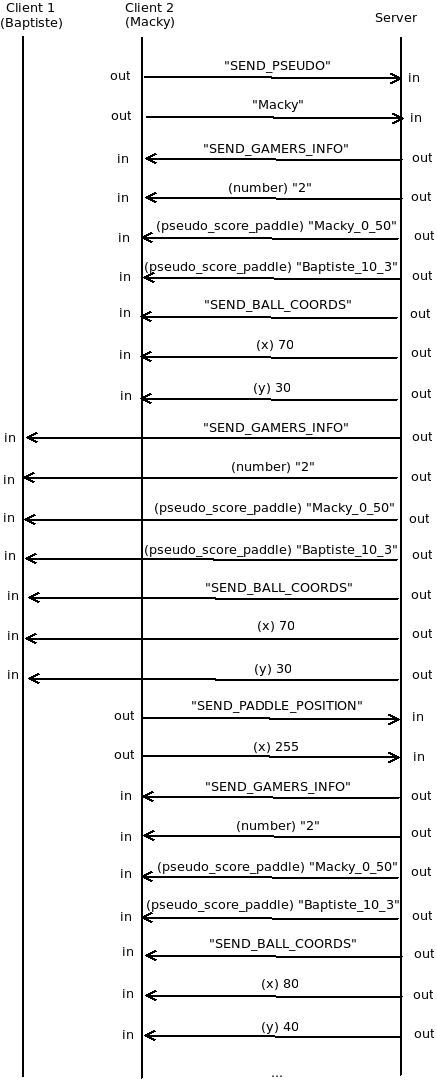
\includegraphics[scale=.45]{protocole.png}
  \end{center}
  \caption{Diagramme de séquence du protocole de communication}
\end{figure}

\newpage

\section{Détails sur le développement}

\textbf{N.B.} Veuillez consulter la Javadoc pour des explications plus précises.

\subsection{Client}

Côté client, le projet est organisé en deux packages (en dehors du main...). À vrai dire, ce ne sont pas de vrais packages au sens strict du terme, car les deux sont intimement liés pour faire fonctionner le jeu. Il était cependant plus clair de séparer la partie purement «~jeu~» de la partie réseau qui gère toutes les interactions avec le serveur.

Dans le package «~game~», on trouve toutes les classes gérant l'interface graphique, ainsi que les éléments du jeu tels que la balle (Ball) ou encore la raquette (Paddle). Concernant l'interface graphique proprement dite, il a fallu étendre les classes de base fournies par Java (JList, JScrollPane, JPanel, ...) pour pouvoir configurer ces composants avec plus de souplesse. Dans la plupart des classes héritées de composants simples Swing, comme par exemple ScoresList ou ScoresZone, on trouve majoritairement un arsenal de constantes et de mutateurs dans le constructeur pour définir les préférences graphiques.

Ceci n'est pas systématique, et on peut le voir notamment avec GameZone où tout s'articule autour de la méthode paintComponent dont la structure a été inspirée du pattern \textbf{Template}. Au sein de cette méthode, on retrouve en effet principalement des appels à d'autres méthodes (en l'occurrence privées), et ces appels définissent la séquence d'exécution du dessin. Ici la séquence a tout de même son importance car il convient de dessiner la zone de jeu avant les autres composants (balle et raquettes). Mais plus généralement, ce découpage au sein de paintComponent rend la méthode beaucoup plus lisible, ce qui permet de mieux visualiser dans le code ce qui est dessiné et dans quel ordre.

On peut le voir aussi avec le cœur de l'interface graphique, soit ClientGUI. La grosse partie se situe ici dans le constructeur où tout le jeu est initialisé côté client. En plus de toutes les configurations d'usage comprenant par exemple le choix du layout (avec le pattern \textbf{Strategy}), on y trouve en particulier un JOptionPane qui permet de rendre le jeu réellement interactif. Lorsque l'utilisateur entre par exemple son pseudo, des contrôles sont lancés pour savoir si celui-ci est valide (au moins 3 caractères). Si c'est le cas, le joueur est autorisé à jouer. Sinon, si le pseudo est invalide ou si l'utilisateur ne veut pas entrer de pseudo, c'est la fin prématurée du jeu.

Pour ce qui est de l'affichage des raquettes notamment, et à des fins ergonomiques, on notera l'utilisation de la méthode setComposite pour gérer la transparence des raquettes adverses. La raquette du joueur courant est, quant à elle, toujours blanche et opaque. Néanmoins, chaque joueur a bel et bien une couleur qui lui est propre dans tout le jeu. On pourra se reporter à la FIGURE 8 en fin de rapport pour avoir un aperçu du rendu.

Par ailleurs, le jeu utilise un certain nombre d'entités qui se traduisent dans le code par des JavaBeans (sans sérialisation), c'est-à-dire des composants simples réutilisables. On peut citer notamment la classe Ball, la classe Paddle, ou encore la classe Gamer, qui sont toutes des classes représentant des entités manipulables. Ces classes définissent toutes un constructeur par défaut sans paramètres et elles respectent toutes le principe d'encapsulation, fournissant de fait des moyens d'accès en lecture et en écriture aux attributs (via des getters et des setters).

Il convient enfin de noter qu'un soin particulier a été apporté au choix du type des constantes dans cette application. Pour éviter d'encombrer inutilement la mémoire, il était souvent plus judicieux d'utiliser des «~byte~» (sur 1 octet) ou des «~short~» (sur 2 octets) que des «~int~» (sur 4 octets).

\subsection{Serveur}

Avant de rentrer dans les détails, il est important de préciser la structure et l'organisation des classes en packages. Côté serveur, les classes de l'application sont séparées en trois packages. Le package game, qui contient toutes les classes concernant le jeu en lui-même (balle, gestionnaire, joueur et raquette)~; le package network, qui contient toutes les classes permettant la communication sur le réseau entre le client et le serveur ; le package principal (main) contenant la classe de lancement du serveur (Main).

Le processus se déroule de la façon suivante~: la classe principale Server contient une ArrayList statique de gestionnaires client (GamerManagement) et reste en écoute permanente de connexions dans une boucle infinie. À chaque fois qu'un client se connecte, le serveur récupère le socket de ce dernier grâce à sa méthode accept. Il instancie et lance ensuite le thread GamerManagement en lui passant le socket qu'il vient d'accepter en paramètre du constructeur. En effectuant cette instanciation, le serveur associe le client à son gestionnaire. Ce gestionnaire est alors ajouté à la liste statique des gestionnaires de clients du serveur, celle-ci étant propre à la classe Server. De ce fait, elle est mise à jour systématiquement à chaque fois qu'un client se connecte.

Dès lors que le gestionnaire du client courant est démarré, celui-ci récupère dans son constructeur l'entrée (getInputStream) et la sortie (getOutputStream) de son client. Cette initialisation était notamment cruciale pour le bon fonctionnement du système. Car par la suite, pour pouvoir envoyer des informations à tous les clients connectés (broadcasting), il fallait impérativement connaître les entrées et sorties standard de chaque client spécifique, et surtout ne pas rester bloqué sur la méthode accept. De plus, on peut noter que le gestionnaire initialise également un objet Gamer, cet objet représentant la référence de joueur qui est associé au client. À ce stade, l'objet Gamer ne contient pas encore de pseudo ni de score, et la raquette (Paddle) contient une valeur par défaut. Chaque objet Gamer contient une référence vers l'objet Paddle qui correspond à sa raquette.

Le thread gérant chaque client (GamerManagement) est chargé de démarrer deux autres threads dans sa méthode run~: Input et Output. Ces deux classes s'occupent respectivement d'écouter les messages du client et d'envoyer des données à ce dernier. La plus grosse partie du code métier du serveur se trouve d'ailleurs dans la classe Output, qui gère la balle et les scores...

Le thread Output contient une méthode helper (moveBall) permettant de gérer le déplacement de la balle. Cette méthode est appelée dans une boucle infinie et possèdent deux booléens : reverseX pour savoir si la balle doit reculer sur l'axe des x et reverseY pour savoir si elle doit reculer sur l'axe des y. Dans cette boucle, nous modifions constamment les coordonnées de la balle grâce à ses setters, et nous détectons les collisions avec les murs et les raquettes selon les principes évoqués dans l'analyse du problème. Quand la balle est perdue, une nouvelle balle avec des coordonnées aléatoires est générée grâce à la méthode createNewBall (qui appelle getRandomCoords en interne).

Pour le calcul des scores, qui dépend des collisions avec les raquettes, le thread Output possède une méthode calculateScore qui met en pratique la formule vue en première partie de ce rapport.

Enfin, de même que pour le client, le serveur prête attention au poids des constantes en utilisant systématiquement le type le moins consommateur de ressources en fonction de l'usage. Si on prend par exemple GameDimensions, qui sert à centraliser toutes les constantes du jeu côté serveur, on constate qu'on n'utilise que des «~byte~» ou des «~short~» car on sait bien que notre jeu doit tenir dans un écran, et donc on sait que 16 bits suffisent largement pour stocker chaque information.

\subsection{Protocole}

Du point de vue du code, le protocole a d'abord été implémenté en utilisant des constantes à l'aide d'une énumération (qui est fatalement la même côté client et côté serveur). Ces constantes correspondent en fait aux primitives évoquées plus haut.

Concrètement, le développement du protocole se trouve dans le package network, que ce soit côté client ou côté serveur. En particulier, on retrouve ce protocole dans les threads gérant les entrées/sorties (Input \& Output). Dans ces threads, des tests sont réalisés en continu dans une boucle infinie pour connaître la primitive transmise. Ces tests permettent notamment d'effectuer des actions spécifiques en fonction de la primitive. Par exemple, si le client envoie «~SEND\_PSEUDO~» au serveur, il faut que l'information qui suive soit le pseudo, et pas les coordonnées de la raquette...

Le protocole s'appuie surtout sur des classes fournies par Java, à savoir un BufferedReader pour les entrées (in) et un PrintWriter pour les sorties (out). Ces classes viennent d'ailleurs décorer (pattern \textbf{Decorator}) les traditionnels InputStream et OutputStream, plus rudimentaires. \textit{In fine}, le client et le serveur ne s'échangent des informations qu'au travers de simples out.println() et in.readline(). Toutes les données sont alors envoyées sous forme de chaîne de caractères ; y compris les nombres, comme par exemple les coordonnées de la balle. Bien sûr, on s'assure ensuite de manipuler les bons types en castant les chaînes reçues quand cela s'avère nécessaire.

\textbf{Attention à la lecture du protocole dans le code !} Par convention, nous avons opté uniquement pour des primitives de type SEND décrivant un envoi d'information, de part et d'autre. Autrement dit, il est normal de voir des SEND à la fois dans Input \& Output. Les SEND dans Input sont les primitives écoutées, tandis que les SEND dans Output sont réellement utilisées pour l'envoi.

\begin{landscape}
  \begin{figure}
  \begin{center}
    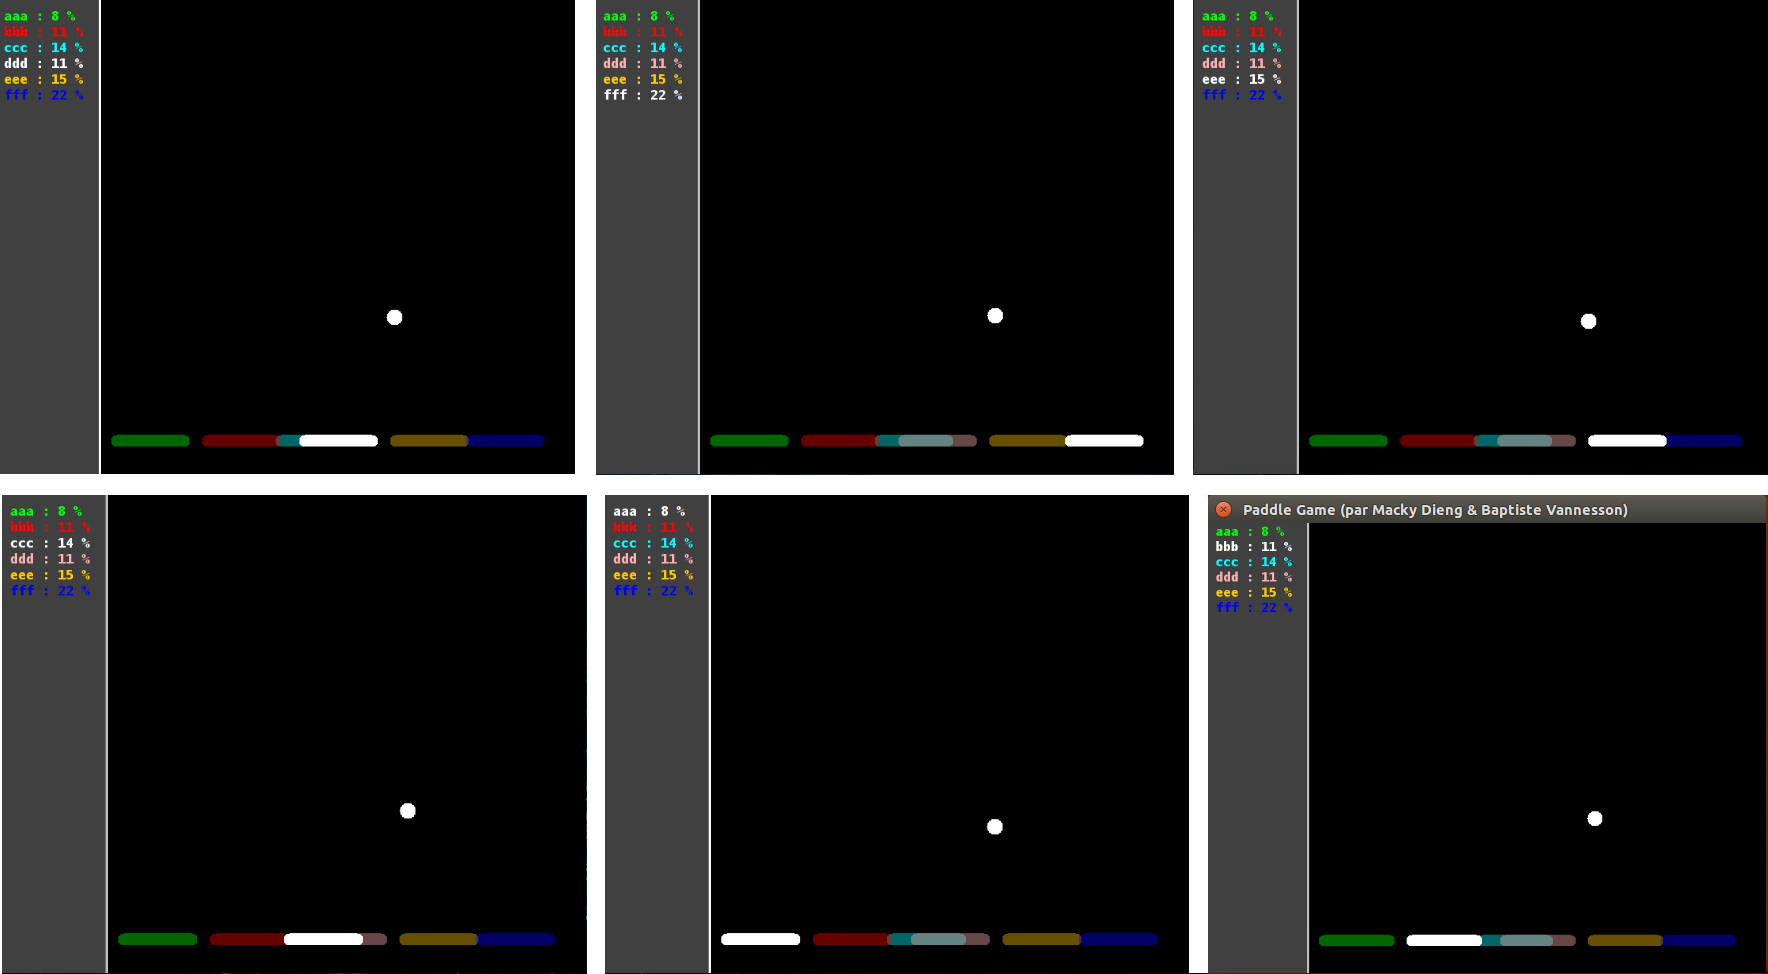
\includegraphics[scale=.3]{multiplayer.png}
  \end{center}
  \caption{Jeu en pleine action, avec plusieurs joueurs}
  \end{figure}
\end{landscape}

\end{document}
